%%%%%%%%%%%%%%%%%%%%%%%%%%%%%%%%%%%%%%%%%%%%%%%%%%%%%%%%%
%                                                       %
% Vorlage fuer die Erstellung einer Abschlussarbeit     %
% im Corporate Design der Universität Konstanz          %
% Stand: 14.09.2016 - Michael Brendle (Version 0.4)     %
%                                                       %
%%%%%%%%%%%%%%%%%%%%%%%%%%%%%%%%%%%%%%%%%%%%%%%%%%%%%%%%%


% Dies ist eine Beispiel für das Erstellen einer
% Abschlussarbeit mit, und ohne, der Systemschrift Arial
% (XeLaTeX oder PDFLatex) im Corporate Design der
% Universität Konstanz.
%
% Dieses Beispieldokument soll so viele Szenarien
% wie möglich abdecken, von Aufzählungen, Listen, Tabellen,
% Kapitel, Abschnitten, Fußnoten, Kopfzeilen, Schriftgrößen
% Abbildungen, Corporate Design Elemente wie Markieren,
% Unterstreichen und Merken, sowie weitere grafische
% Elemente im Corporate Design die zur Gestaltung
% verwendet werden können (Block, Pfeile, Linien und
% Klammern).
%
% Für weitere Informationen sei auch zur README.txt in
% diesem Ordner verwiesen.
%
% Sollten Sie Probleme beim Kompilieren haben, können
% Sie dieses Dokument auch online, in Overleaf, unter
% der URL
%
%    https://www.overleaf.com/6205861nhvynn
%
% einsehen, bearbeiten und kompilieren.
%
% Schauen Sie, dass Ihre Tex-Distribution, sowie alle Pakete
% auf dem aktuellsten Stand sind, um Probleme zu vermeiden.



%%%%%%%%%%%%%%%%%%%%%%%%%%%%%%%%%%%%%%%%%%%%%%%%%%%%%%%%%
% Dokumentenklasse scrreprt         ja                    %
%%%%%%%%%%%%%%%%%%%%%%%%%%%%%%%%%%%%%%%%%%%%%%%%%%%%%%%%%

\documentclass[ngerman, 11pt, rgb]{scrreprt}



%%%%%%%%%%%%%%%%%%%%%%%%%%%%%%%%
% Paket Theme Konstanz         %
%%%%%%%%%%%%%%%%%%%%%%%%%%%%%%%%

% Alle verwendeten Makros und Umgebeungen, die zur Erstellung von
% PDF-Dokumenten und Abschlussarbeiten benötigt werden, können
% aus dem Paket themeKonstanz geladen werden, welches sich in der
% Datei themeKonstanz.sty befindet.
%
% Möchte man dieses Dokument mit XeLaTeX anstatt PDFLatex kompilieren,
% um die Systemschrift Arial zu verwenden, dann muss zusätzlich das
% Add-On Paket themeKonstanzXelatexAddOn, welches sich in der Datei
% themeKonstanzXelatexAddOn.sty befindet VOR dem eigentlichen
% Paket themeKonstanz geladen werden (siehe unten).
%
% Möchte man ein Style Add-On verwenden, das aus meiner
% Bachelorarbeit aus dem Jahr 2015 stammt, so muss NACH dem Laden
% des Paketes themeKonstanz dieses zusätzliche Paket
% themeKonstanzStyleAddOn, welches sich in der Datei
% themeKonstanzStyleAddOn.sty befindet, geladen werden. Dabei
% werden die Überschriften der Kapitel, der Abschnitte, der Unter-
% Abschnitte und des Unterunterabschnittes geändert. Dieses
% Add-On wird vor allem für Abschlussarbeiten empfohlen, die
% nicht zu farbig sein sollten und nicht so strikt an das
% Corporate Design der Universität Konstanz gebunden sind.

%\usepackage{themeKonstanzXelatexAddOn} % XeLaTeX mit Schriftart Arial, VOR dem Standardpaket importieren
\usepackage{themeKonstanz} % Muss immer verwendet werden (Standardpaket)
%\usepackage{themeKonstanzStyleAddOn} % Style Add-On für andere Überschriften, NACH dem Standardpaket importieren



%%%%%%%%%%%%%%%%%%%%%%%%%%%%%%%%
% Papierformat                 %
%%%%%%%%%%%%%%%%%%%%%%%%%%%%%%%%

% Mit Hilfe des Makros
%
%    \format{<key>}
%
% kann das Papierformat angepasst werden.
%
% Zur Auswahl stehen folgende Papierformate:
%
%   Schlüssel  Beschreibung      Höhe      Breite
%   -----------------------------------------------
%   a3         DinA3 Hochformat  42.0  cm  29.7  cm
%   a3quer     DinA3 Querformat  29.7  cm  42.0  cm
%   a4         DinA4 Hochformat  29.7  cm  21.0  cm
%   a4quer     DinA4 Querformat  21.0  cm  29.7  cm
%   a5         DinA5 Hochformat  21.0  cm  14.8  cm
%   a5quer     DinA5 Querformat  14.8  cm  21.0  cm
%
% Falls keiner der unterstützten Schlüssel übergeben wird,
% ist DinA4 Hochformat der Standard.

% Wähle hier DinA4 Hochformat mit dem Schlüssel a4 aus.

\format{a4}



%%%%%%%%%%%%%%%%%%%%%%%%%%%%%%%%
% Dokumentinformationen        %
%%%%%%%%%%%%%%%%%%%%%%%%%%%%%%%%

% Für das Dokument können mit Hilfe der Makros
%
%    \date{...}
%    \year{...}
%    \author{...}
%    \title{...}
%    \subtitle{...}
%    \unisection{...}
%    \department{...}
%    \supervisorOne{...}
%    \supervisorTwo{...}
%
% das Datum, das Jahr, der Autor / die Autoren, der Titel, der
% Unteritel des Dokumentes, die Sektion an der Universität,
% der Fachbereich an der Universität, der Erstgutachter und der
% Zweitgutachter bestimmt werden.
%
% Je nachdem, ob die Corporate Design Titelseite oder die
% Thesis-Titelseite ausgewählt wird, werden die entsprechenden
% Angaben dargestellt und verwendet. Außerdem benutzen die
% Kopf- und Fusszeile diese Informationen (siehe weiter unten).

\date{31.10.2018}
\year{2018}
\author{Hermann B\"ottcher \& Jannik Dornseiff}
\title{Laserspektroskopie}
\subtitle{Untertitel des Dokuments}
\unisection{Mathematisch-Naturwissenschaftlichen Sektion}
\department{Fachbereich Physik}
\supervisorOne{Timo Raab}



%%%%%%%%%%%%%%%%%%%%%%%%%%%%%%%%
% Kopf und Fusszeile           %
%%%%%%%%%%%%%%%%%%%%%%%%%%%%%%%%

% Mit Hilfe des Makros
%
%    \headFoot
%
% kann aus 20 vordefinierten Kopf- und Fusszeilen
% gewählt werden.
%
% Dieses Makro besitzt ein Argument, nämlich die
% ID aus den 20 vordefinierten Kopf- und Fusszeilen:
%
%    \headFoot{<ID>}
%
% Bei den IDs 1, 2, 5, 6, 9, 10, 13, 14, 17 und 18
% mit | wird auf ungerade und gerade Seite geachtet.
%
% Bei den restlichen IDs ist die Kopf- und Fusszeile auf
% ungeraden und geraden Seiten gleich.
%
% Dies soll vor allem dem Benutzer die Entscheidung
% überlassen, ob er das Dokument einseitig oder doppelseitig
% ausdruckt.
%
%
%   ID    Beschreibung
%   ------------------
%   1     Kopfzeile: Seite --- Kapitel --- Autor | Autor --- Kapitel --- Seite
%         Fusszeile:
%
%   2     Kopfzeile:
%         Fusszeile: Seite --- Kapitel --- Autor | Autor --- Kapitel --- Seite
%
%   3     Kopfzeile: Autor --- Kapitel --- Seite
%         Fusszeile:
%
%   4     Kopfzeile:
%         Fusszeile: Autor --- Kapitel --- Seite
%
%   5     Kopfzeile: Seite --- Autor --- Kapitel | Kapitel --- Autor --- Seite
%         Fusszeile:
%
%   6     Kopfzeile:
%         Fusszeile: Seite --- Autor --- Kapitel | Kapitel --- Autor --- Seite
%
%   7     Kopfzeile: Kapitel --- Autor --- Seite
%         Fusszeile:
%
%   8     Kopfzeile:
%         Fusszeile: Kapitel --- Autor --- Seite
%
%   9     Kopfzeile: Seite --- --- Kapitel | Name --- --- Seite
%         Fusszeile:
%
%   10    Kopfzeile:
%         Fusszeile: Seite --- --- Kapitel | Name --- --- Seite
%
%   11    Kopfzeile: Kapitel --- --- Seite
%         Fusszeile:
%
%   12    Kopfzeile:
%         Fusszeile: Kapitel --- --- Seite
%
%   13    Kopfzeile: Seite --- --- Autor | Kapitel --- --- Seite
%         Fusszeile:
%
%   14    Kopfzeile:
%         Fusszeile: Seite --- --- Autor | Kapitel --- --- Seite
%
%   15    Kopfzeile: Autor --- --- Seite
%         Fusszeile:
%
%   16    Kopfzeile:
%         Fusszeile: Autor --- --- Seite
%
%   17    Kopfzeile: Seite --- --- | --- --- Seite
%         Fusszeile:
%
%   18    Kopfzeile:
%         Fusszeile: Seite --- --- | --- --- Seite
%
%   19    Kopfzeile: --- --- Seite
%         Fusszeile:
%
%   20    Kopfzeile:
%         Fusszeile: --- --- Seite
%
% Weitere individuelle Kopf- und Fusszeilen können in der .sty Datei angepasst werden.

% Wähle die ID 14 mit
%    Kopfzeile:
%    Fusszeile: Seite --- --- Autor | Kapitel --- --- Seite

\headFoot{14}



%%%%%%%%%%%%%%%%%%%%%%%%%%%%%%%%%%%%%%%%%%%%%%%%%%%%%%%%%
% Begin vom Dokument                                    %
%%%%%%%%%%%%%%%%%%%%%%%%%%%%%%%%%%%%%%%%%%%%%%%%%%%%%%%%%

\begin{document}

\pagenumbering{Roman}


%%%%%%%%%%%%%%%%%%%%%%%%%%%%%%%%
% Uni-Titelseite               %
%%%%%%%%%%%%%%%%%%%%%%%%%%%%%%%%

% Mit Hilfe des Makros
%
%    \unititlepage
%
% kann die Titleseite des Dokumentes im Corporate Design der
% Universität Konstanz erstellt werden.
%
% Das Makro besitzt drei optionale Argumente, die mit
% Key-Value-Pairs eingesetzt werden können:
%
%    \unititlepage[Optionen mit Key-Value-Pairs]
%
% Dabei stehen folgende Optionen zur Verfügung:
%
%    graphic      Möchte man ein Bild, Grafik, o.ä. auf der
%                 Titelseite platzieren, so muss nur der Pfad
%                 dieser Grafik eingesetzt werden (Beispiel siehe
%                 unten).
%
%                 Wird kein Grafikpfad angegeben oder wird dieses
%                 optionale Argument weggelassen, so wird ein
%                 leeres graues Rechteck entsprechend CD-Richtlinien
%                 erstellt.
%
%    partnerlogo  Möchte man ein Partner- bzw. Zweitlogo auf der
%                 Titelseite platzieren, so muss auch hier der
%                 Pfad angegeben werden, und es wird in der linken
%                 oberen Ecke platziert (Beispiel siehe unten).
%
%                 Wird dieses optionale Argument weggelassen, so wird
%                 an dieser Stelle natürlich kein Logo präsentiert.
%
%    unilogo      Standardmäßig wird in der rechten oberen Ecke auf
%                 der Titelseite das Unilogo platziert.
%
%                 Möchte man an dieser Stelle ein anderes Logo, so muss
%                 auch hier der Pfad angegeben werden. Dies sollte jedoch
%                 nur in besonderen Fällen erfolgen, da das Uni-Logo nach
%                 CD Richtlinien i.d.R. in der oberen rechten Ecke
%                 platziert werden sollte.
%
%                 Wird das optionale Argument verwendet, jedoch kein Pfad
%                 angegeben, so wird auch kein Logo in der rechten oberen
%                 Ecke angezeigt.
%
%                 Wird das optionale Argument weggelassen, so wird
%                 standardmäßig das Uni-Logo in der rechten oberen
%                 Ecke präsentiert.

%\unititlepage[graphic=graphics/indoor_sw, partnerlogo=graphics/PHTG_logo]%



%%%%%%%%%%%%%%%%%%%%%%%%%%%%%%%%
% Thesis-Titelseite            %
%%%%%%%%%%%%%%%%%%%%%%%%%%%%%%%%

% Mit Hilfe des Makros
%
%    \thesistitlepage
%
% kann die Titleseite des Dokumentes an die Vorgaben
% einer Arbeit (Bachelorarbeit, Masterarbeit, ... ) des
% Fachbereichs Informatik und Informationswissenschaft
% angepasst werden.
%
% Das Makro besitzt ein festes und ein optionales Argument.
%
%    \unititlepage[language=<language>]{<Art der Arbeit>}
%
% Dabei stehen folgende Optionen zur Verfügung:
%
%    language        Mit diesem Optionalen Argument kann die
%                    Sprache der Titelseite angepasst werden.
%
%                    Mögliche Werte sind
%
%                        german
%                        english
%
%                    Je nach dem übergebenen Wert, wird die Titelseite
%                    entweder auf Deutsch oder English erstellt.
%
%                    Sollte diese Option weggelassen werden, wird
%                    die Titelseite auf Deutsch erstellt.
%
%    Art der Arbeit  Hier kann die Art der Arbeit übergeben werden,
%                    welche auf der Titelseite erscheint.
%
%                    Hier kann alles übergeben werden. Normalerweise
%                    wird hier Bachelorarbeit, Masterarbeit, o.ä.
%                    angegeben.
%
% Diese Thesis-Titelseite ist auf DinA4 Hochformat optimiert!

\thesistitlepage[language=german]{Fortgeschrittenenpraktikumsbericht}



%%%%%%%%%%%%%%%%%%%%%%%%%%%%%%%%
% Inhaltsverzeichnis           %
%%%%%%%%%%%%%%%%%%%%%%%%%%%%%%%%

% Das Inhaltsverzeichnis kann wie gewohnt mit dem Makro
%
%    \tableofcontents
%
% erstellt werden.

\begin{abstract}
  In diesem Versuch wird ein Teil des Termschemas von $\mathrm{^{133}Cs}$ untersucht. Das Augenmerk liegt hierbei auf der Hyperfeinstruktur der Niveaus $6^2S_{1/2}$ und $6^2P_{3/2}$. Zu dessen Charakterisierung werden sowohl dopplerverbreiterte, als auch dopplerfreie Transmissionspektren einer C\"asiumgaskammer aufgenommen. Hierbei kommen ein Diodenlaser und außerdem, zu Zwecken der Kalibrierung, ein Fabry-Pert-Etalon zum Einsatz.

  Zunächst wird die Linienbreite des Lasers zu $\SI{11,14(25)}{\mega\hertz}$ bestimmt. Der experimentell bestimmte Wert der Sekunde ist $\SI{0,90(1)}{\second}$. Das Termschema von C\"asium ergibt sich mit den Ergebnissen wie unten abgebildet.\\


  \begin{centering}

  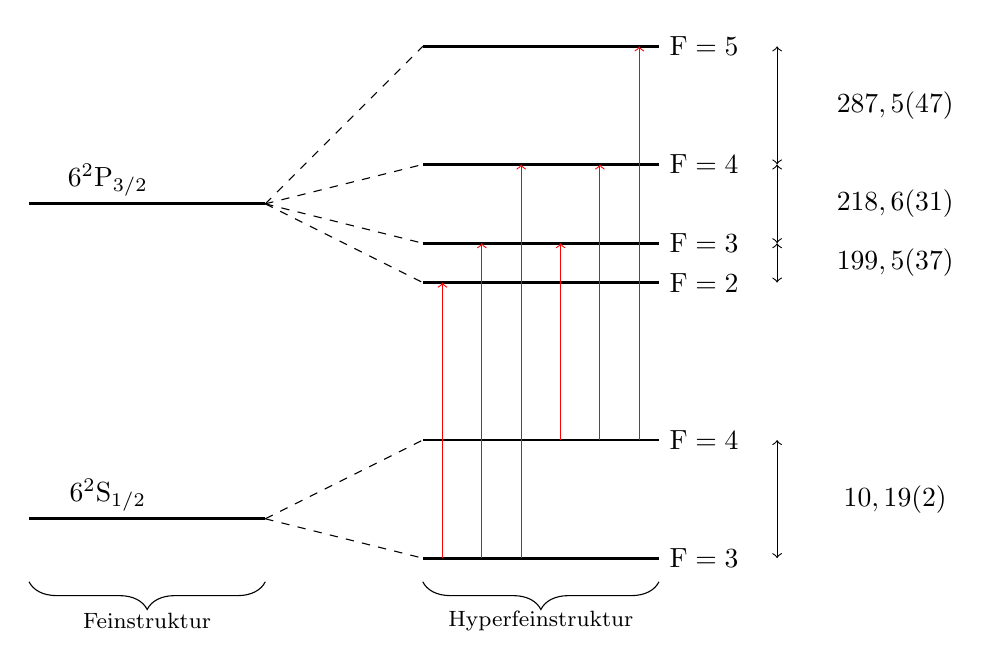
\begin{tikzpicture}
    % angeregte Niveaus
    \node at (1,4.3) {$\mathrm{6^2P_{3/2}}$};
    \draw[line width=1pt] (0,4)--(3,4);
    \draw[line width=1pt] (5,6)--(8,6) node[anchor=west] {$\mathrm{F=5}$};
    \draw[line width=1pt] (5,4.5)--(8,4.5) node[anchor=west] {$\mathrm{F=4}$};
    \draw[line width=1pt] (5,3.5)--(8,3.5) node[anchor=west] {$\mathrm{F=3}$};
    \draw[line width=1pt] (5,3)--(8,3) node[anchor=west] {$\mathrm{F=2}$};
    \draw[dashed] (3,4)--(5,6);
    \draw[dashed] (3,4)--(5,4.5);
    \draw[dashed] (3,4)--(5,3.5);
    \draw[dashed] (3,4)--(5,3);
    % Grundzustand Niveaus
    \node at (1,0.3) {$\mathrm{6^2S_{1/2}}$};
    \draw[line width=1pt](0,0)--(3,0);
    \draw[line width=1pt] (5,1)--(8,1) node[anchor=west] {$\mathrm{F=4}$};
    \draw[line width=1pt] (5,-0.5)--(8,-0.5) node[anchor=west] {$\mathrm{F=3}$};
    \draw[dashed] (3,0)--(5,1);
    \draw[dashed] (3,0)--(5,-0.5);
    % \"Uberg\"ange
    % Unterer Grundzustand
    \draw[color=red, ->] (5.25,-0.5)--(5.25,3);
    \draw[color=red, ->] (5.75,-0.5)--(5.75,3.5);
    \draw[color=red, ->] (6.25,-0.5)--(6.25,4.5);
    % Oberer Grundzustand
    \draw[color=red, ->] (6.75,1)--(6.75,3.5);
    \draw[color=red, ->] (7.25,1)--(7.25,4.5);
    \draw[color=red, ->] (7.75,1)--(7.75,6);
    % Messwerte
    \draw[<->] (9.5,-0.5)--(9.5,1);
    \node at (11,0.25) {$\SI{10,19(2)}{\giga\hertz}$};
    \draw[<->] (9.5,3)--(9.5,3.5);
    \node at (11,3.25) {$\SI{199,5(37)}{\mega\hertz}$};
    \draw[<->] (9.5,3.5)--(9.5,4.5);
    \node at (11,4) {$\SI{218,6(31)}{\mega\hertz}$};
    \draw[<->] (9.5,4.5)--(9.5,6);
    \node at (11,5.25) {$\SI{287,5(47)}{\mega\hertz}$};
    % Fein- und Hyperfeinstruktur
    \draw [decorate,decoration={brace,mirror,amplitude=10pt}] (0,-0.8) -- (3,-0.8) node [black,midway,yshift=-14pt] {\footnotesize Feinstruktur};
    \draw [decorate,decoration={brace,mirror,amplitude=10pt}] (5,-0.8) -- (8,-0.8) node [black,midway,yshift=-14pt] {\footnotesize Hyperfeinstruktur};
  \end{tikzpicture}
\end{centering}
\end{abstract}

\tableofcontents



%%%%%%%%%%%%%%%%%%%%%%%%%%%%%%%%
% Abbildungsverzeichnis        %
%%%%%%%%%%%%%%%%%%%%%%%%%%%%%%%%

% Das Abbildungsverzeichnis kann wie gewohnt mit dem Makro
%
%    \listoffigures
%
% erstellt werden.
%
% Möchte man das Abbildungsverzeichnis zum Inhaltsverzeichnis
% hinzufügen, so kann dies mit dem Makro
%
%    \addcontentsline{toc}{chapter}{Abbildungsverzeichnis}
%
% hinzugefügt werden.

\listoffigures
\addcontentsline{toc}{chapter}{Abbildungsverzeichnis}



%%%%%%%%%%%%%%%%%%%%%%%%%%%%%%%%
% Tabellenverzeichnis          %
%%%%%%%%%%%%%%%%%%%%%%%%%%%%%%%%

% Das Tabellenverzeichnis kann wie gewohnt mit dem Makro
%
%    \listoftables
%
% erstellt werden.
%
% Möchte man das Tabellenverzeichnis zum Inhaltsverzeichnis
% hinzufügen, so kann dies mit dem Makro
%
%    \addcontentsline{toc}{chapter}{Tabellenverzeichnis}
%
% hinzugefügt werden.

\listoftables
\addcontentsline{toc}{chapter}{Tabellenverzeichnis}



%%%%%%%%%%%%%%%%%%%%%%%%%%%%%%%%
% Kapitel, Abschnitte, ...     %
%%%%%%%%%%%%%%%%%%%%%%%%%%%%%%%%

% Kapitel, Abschnitte, Unterabschitte und Unterunterabschnitte
% können wie gewohnt mit den Makros
%
%    \chapter{...}
%    \section{...}
%    \subsection{...}
%    \subsubsection{...}
%
% erstellt werden.
%
% Diese werden dann nach den Corporate Design Richtlinien der
% Univeristät Konstanz erstellt.
%
% Sollte das Style Add-on geladen werden, werden alternative
% Überschriften erstellt, die nicht mehr den CD-Richtlinen
% der Universität Konstanz entsprechen, jedoch für Abschluss-
% arbeiten verwendet werden können.



%\rmfamily % Auskommentieren für eine Schrift mit serifen / Kommentieren für eine serifenlose Schrift
\normalsize

\newpage
\pagenumbering{arabic}

%\subfile{kapitel/physikalische_grundlagen.tex}
\subfile{kapitel/einleitung.tex}
\subfile{kapitel/versuch.tex}

\printbibliography
\addcontentsline{toc}{chapter}{Bibliographie}

\subfile{kapitel/anhang.tex}

%%%%%%%%%%%%%%%%%%%%%%%%%%%%%%%%%%%%%%%%%%%%%%%%%%%%%%%%%
% Ende vom Dokument                                     %
%%%%%%%%%%%%%%%%%%%%%%%%%%%%%%%%%%%%%%%%%%%%%%%%%%%%%%%%%

\end{document}
